\section{Mochamad Arifqi Ramadhan (1174074)}
\subsection{Kordinat}
\begin{itemize}
	\item Pengertian Kordinat
	kordinat pada pemetaan adalah pertemuan antara garis bujur (Garis garis lurus atau vertikal pada peta) dan garis lintang (Garis mendatar atau horizontal pada peta). Artinya dalam peta kita akan menemukan garis melintang dan mebujur yang membagi peta menjadi kotak-kotak persegi.
Garis yang melintang dari kiri ke kanan peta disebut Garis Lintang (Latitude), sedangkan garis yang membujur dari atas ke bawah peta disebut Garis Bujur (Longitude).
Bersama, Garis Lintang dan Garis Bujur membentuk sistem koordinat peta.

Garis Lintang digunakan untuk menandai posisi utara-selatan sebuah lokasi di permukaan bumi. Garis Lintang berkisar dari 0 derajat di khatulistiwa sampai 90 derajat Lintang Utara di Kutub Utara dan 90 derajat Lintang Selatan di kutub Selatan.

Sementara itu Garis Bujur digunakan untuk menandai posisi utara-selatan sebuah lokasi di permukaan bumi. Garis Bujur 0 derajat terletak di kota Greenwich, Inggris, dan bergerak sejauh 180 derajat ke barat dan timur, yang bertemu pada titik 180 derajat di tengah Samudera Pasifik. Jarak antara masing-masing derajat garis lintang kira-kira 69 mil (111 km).

Contoh koordinat dengan Garis Lintang dan Garis Bujur ini adalah kota Jakarta dengan lokasi terletak di 6,2 derajat Lintang Selatan dan 107 derajat Bujur Timur.

\item Sejarah Kordinat
	
Konsep sudut dan jari-jari sudah digunakan oleh manusia sejak zaman purba, paling tidak pada milenium pertama SM. Astronom dan astrolog Yunani, Hipparchus, (190–120 SM) menciptakan tabel fungsi chord dengan menyatakan panjang chord bagi setiap sudut, dan ada rujukan mengenai penggunaan koordinat polar olehnya untuk menentukan posisi bintang-bintang.[2] Dalam karyanya On Spirals, Archimedes menyatakan Archimedean spiral, suatu fungsi yang jari-jarinya tergantung dari sudut. Namun, karya-karya Yunani tidak berkembang sampai ke suatu sistem koordinat sepenuhnya.

Dari abad ke-8 M dan seterusnya, para astronom mengembangkan metode untuk menghitung arah ke Mekkah (kiblat)— dan jaraknya — dari semua lokasi di bumi

	\item Sistem Kordinat 
Sistem kordinat merupakan suatu parameter yang menunjukkan bagaimana suatu objek diletakkan dalam koordinat. Ada 3 sistem kordinat yang digunakan dalam pemetaan, antara lain :


	\begin{enumerate}
	\item Sistem Koordinat 1 Dimensi
	
	\begin{figure}[H]
	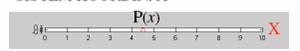
\includegraphics[width=4cm]{figures/Tugas1/1174074/dimensi1.jpg}
	\centering
	\caption{Gambar 1}
\end{figure}
	
	\item Sistem Koordinat 2 Dimensi 

	\begin{figure}[H]
	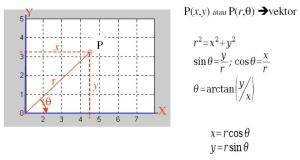
\includegraphics[width=4cm]{figures/Tugas1/1174074/dimensi2.jpg}
	\centering
	\caption{Gambar 1}
\end{figure}

\item Sistem Koordinat 3 Dimensi

	\begin{figure}[H]
	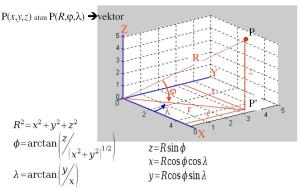
\includegraphics[width=4cm]{figures/Tugas1/1174074/dimensi3.jpg}
	\centering
	\caption{Gambar 1}
\end{figure}

	\end{enumerate}
\end{itemize}
\subsection{Link}
https://youtu.be/5nS7ewD8DQU
\subsection{Plagiarism}
\begin{figure}[H]
	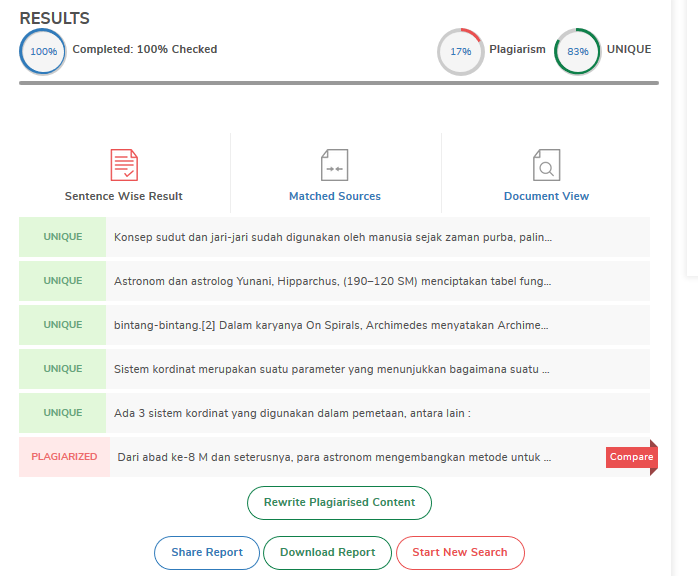
\includegraphics[width=4cm]{figures/Tugas1/1174074/plagiat.png}
	\centering
	\caption{Gambar Plagiat}
\end{figure}

	
